\documentclass[a4paper]{article}

\usepackage[utf8]{inputenc}
\usepackage{microtype}
\usepackage{enumitem}
\usepackage{comment}
\usepackage{float, graphicx}
\usepackage{mathtools, amssymb}
\usepackage{caption}
\usepackage{subcaption}

\setlength{\parindent}{0em}
\graphicspath{ {../images/} }

\title{5}
\date{}

\begin{document}
\maketitle

\section{Part-a}
Control points were selected as mentioned. Care was taken to select salient features such as easily identifiable points and corners.

\section{Part-b}
The code to calculate the affine matrix can be found inside the code directory. The affine matrix was calculated by using P1 and P2 matrices consisting of control points for image1 and imag2  and finding the pseudo inverse of P1.


\section{Part-c}
The nearest neighbor approximation has been implemented and can be seen in the code section.
The Images are:



\begin{figure}[H]
\begin{subfigure}{.4\textwidth}
  \centering
  % include first image
  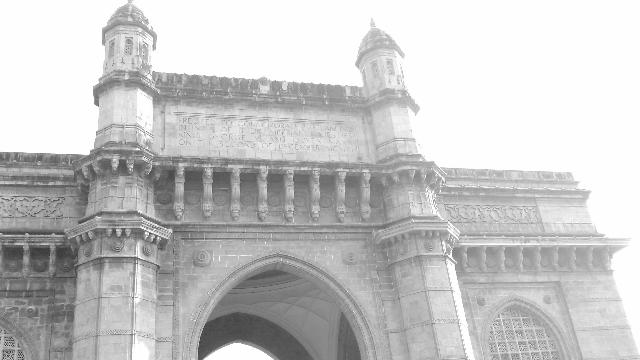
\includegraphics[width=.8\linewidth]{goi1.jpg}  
  \caption{goi1}
  
\end{subfigure}
\begin{subfigure}{.4\textwidth}
  \centering
  % include second image
  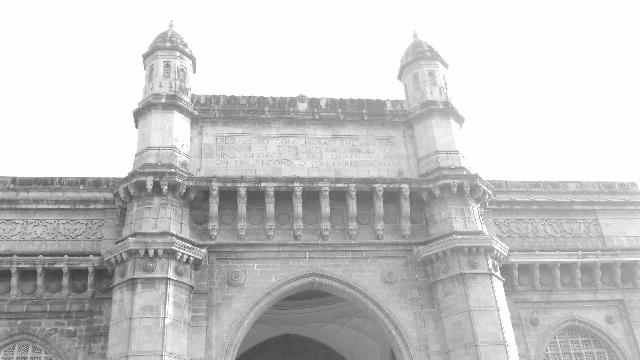
\includegraphics[width=.8\linewidth]{goi2_downsampled.jpg}  
  \caption{goi2}
  
\end{subfigure}



\begin{subfigure}{.4\textwidth}
  \centering
  % include third image
  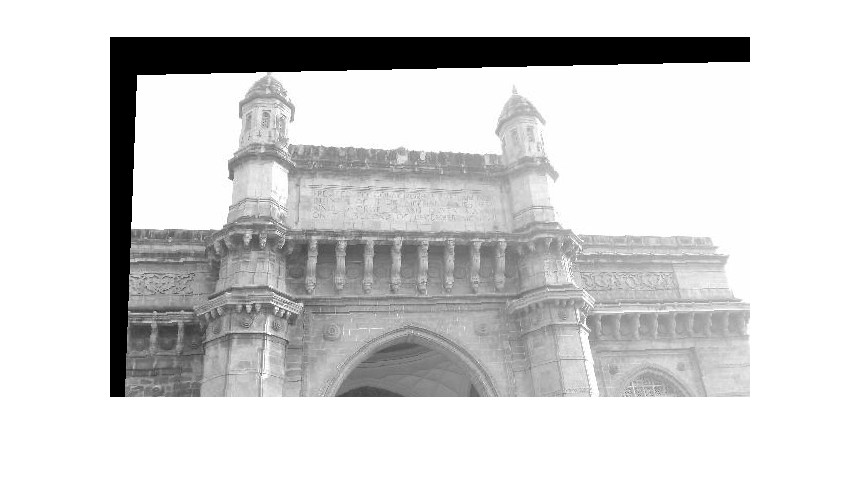
\includegraphics[width=.8\linewidth]{nearest_neighbour.jpg}  
  \caption{nearest-neighbour}
  
\end{subfigure}
\begin{subfigure}{.4\textwidth}
  \centering
  % include fourth image
  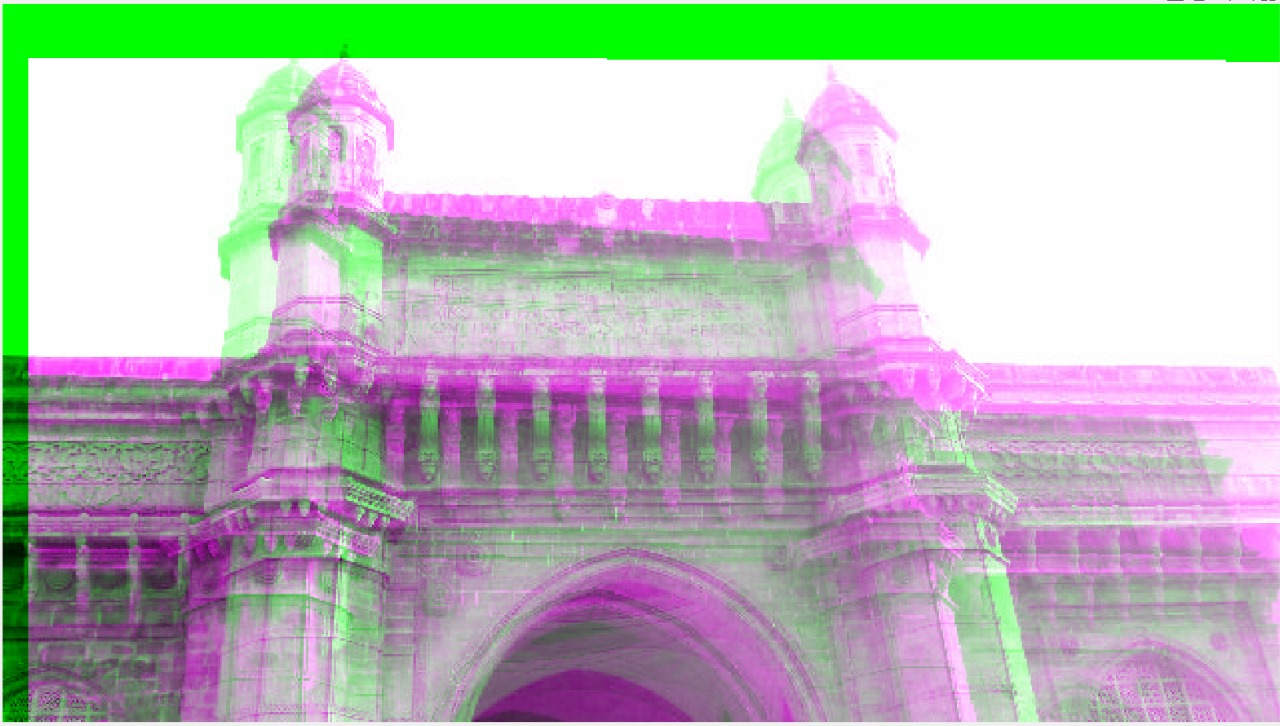
\includegraphics[width=.8\linewidth]{n-12.jpg}  
  \caption{overlay}
  
\end{subfigure}
\caption{Nearest Neighbour}

\end{figure}


\section{Part-d}
The Bi-linear approximation has been implemented and can be seen in the code section.
The Images are:

\begin{figure}[H]
\begin{subfigure}{.4\textwidth}
  \centering
  % include first image
  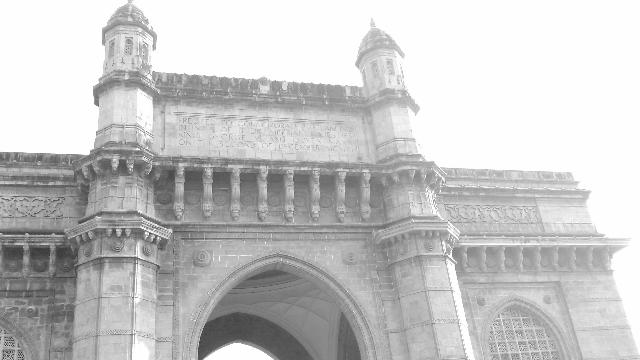
\includegraphics[width=.8\linewidth]{goi1.jpg}  
  \caption{goi1}
  
\end{subfigure}
\begin{subfigure}{.4\textwidth}
  \centering
  % include second image
  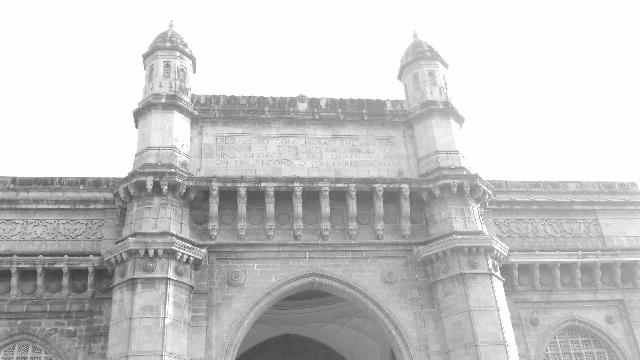
\includegraphics[width=.8\linewidth]{goi2_downsampled.jpg}  
  \caption{goi2}
  
\end{subfigure}



\begin{subfigure}{.4\textwidth}
  \centering
  % include third image
  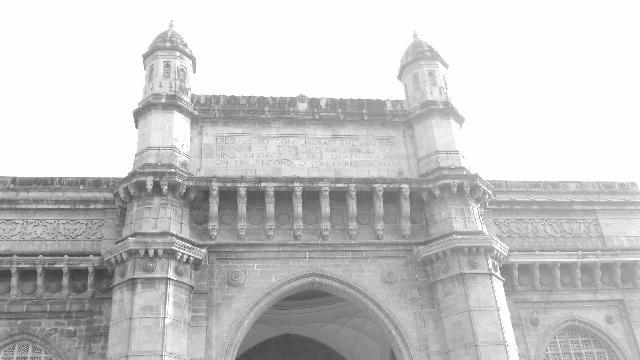
\includegraphics[width=.8\linewidth]{b.jpg}  
  \caption{Bi-linear}
  
\end{subfigure}
\begin{subfigure}{.4\textwidth}
  \centering
  % include fourth image
  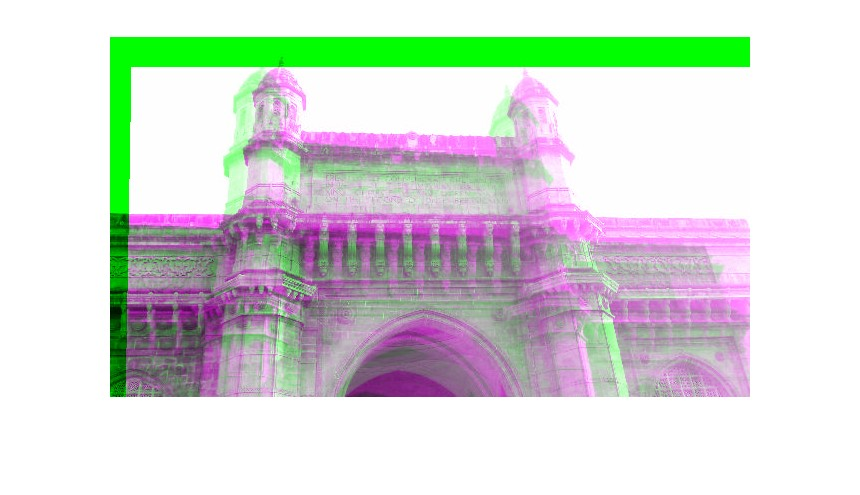
\includegraphics[width=.8\linewidth]{ob.jpg}  
  \caption{overlay}
  
\end{subfigure}
\caption{Bi-linear}

\end{figure}





\end{document}
